%%%%%%%%%%%%%%%%%%%%%%%%%%%%%%%%%%%%%%%%%
% Beamer Presentation
% LaTeX Template
% Version 1.0 (10/11/12)
%
% This template has been downloaded from:
% http://www.LaTeXTemplates.com
%
% License:
% CC BY-NC-SA 3.0 (http://creativecommons.org/licenses/by-nc-sa/3.0/)
%
%%%%%%%%%%%%%%%%%%%%%%%%%%%%%%%%%%%%%%%%%

%----------------------------------------------------------------------------------------
%	PACKAGES AND THEMES
%----------------------------------------------------------------------------------------

\documentclass{beamer}

\mode<presentation> {

% The Beamer class comes with a number of default slide themes
% which change the colors and layouts of slides. Below this is a list
% of all the themes, uncomment each in turn to see what they look like.

%\usetheme{default}
%\usetheme{AnnArbor}
%\usetheme{Antibes}
%\usetheme{Bergen}
%\usetheme{Berkeley}
%\usetheme{Berlin}
%\usetheme{Boadilla}
%\usetheme{CambridgeUS}
%\usetheme{Copenhagen}
%\usetheme{Darmstadt}
%\usetheme{Dresden}
%\usetheme{Frankfurt}
%\usetheme{Goettingen}
%\usetheme{Hannover}
%\usetheme{Ilmenau}
%\usetheme{JuanLesPins}
%\usetheme{Luebeck}
\usetheme{Madrid}
%\usetheme{Malmoe}
%\usetheme{Marburg}
%\usetheme{Montpellier}
%\usetheme{PaloAlto}
%\usetheme{Pittsburgh}
%\usetheme{Rochester}
%\usetheme{Singapore}
%\usetheme{Szeged}
%\usetheme{Warsaw}

% As well as themes, the Beamer class has a number of color themes
% for any slide theme. Uncomment each of these in turn to see how it
% changes the colors of your current slide theme.

%\usecolortheme{albatross}
%\usecolortheme{beaver}
%\usecolortheme{beetle}
%\usecolortheme{crane}
%\usecolortheme{dolphin}
%\usecolortheme{dove}
%\usecolortheme{fly}
%\usecolortheme{lily}
%\usecolortheme{orchid}
%\usecolortheme{rose}
%\usecolortheme{seagull}
%\usecolortheme{seahorse}
%\usecolortheme{whale}
%\usecolortheme{wolverine}

%\setbeamertemplate{footline} % To remove the footer line in all slides uncomment this line
%\setbeamertemplate{footline}[page number] % To replace the footer line in all slides with a simple slide count uncomment this line

%\setbeamertemplate{navigation symbols}{} % To remove the navigation symbols from the bottom of all slides uncomment this line
}

\usepackage{graphicx} % Allows including images
\usepackage{booktabs} % Allows the use of \toprule, \midrule and \bottomrule in tables
\usepackage[brazilian]{babel}
\usepackage[utf8]{inputenc}
\usepackage[T1]{fontenc}
\usepackage{amsmath}
\usepackage{hyperref}
\usepackage{url}
% Default fixed font does not support bold face
\DeclareFixedFont{\ttb}{T1}{txtt}{bx}{n}{12} % for bold
\DeclareFixedFont{\ttm}{T1}{txtt}{m}{n}{12}  % for normal

% Custom colors
\usepackage{color}
\definecolor{deepblue}{rgb}{0,0,0.5}
\definecolor{deepred}{rgb}{0.6,0,0}
\definecolor{deepgreen}{rgb}{0,0.5,0}

\usepackage{listings}

% Python style for highlighting
\newcommand\pythonstyle{\lstset{
language=Python,
basicstyle=\ttm,
otherkeywords={self},             % Add keywords here
keywordstyle=\ttb\color{deepblue},
emph={MyClass,__init__},          % Custom highlighting
emphstyle=\ttb\color{deepred},    % Custom highlighting style
stringstyle=\color{deepgreen},
frame=tb,                         % Any extra options here
showstringspaces=false            % 
}}


% Python environment
\lstnewenvironment{python}[1][]
{
\pythonstyle
\lstset{#1}
}
{}

% Python for external files
\newcommand\pythonexternal[2][]{{
\pythonstyle
\lstinputlisting[#1]{#2}}}

% Python for inline
\newcommand\pythoninline[1]{{\pythonstyle\lstinline!#1!}}

\setbeamertemplate{navigation symbols}{}

%----------------------------------------------------------------------------------------
%	TITLE PAGE
%----------------------------------------------------------------------------------------

\title[Deep Learning com Keras]{Modelagem de Redes Neurais Profundas com Keras} % The short title appears at the bottom of every slide, the full title is only on the title page

\author{Caio Jordão Carvalho} % Your name
\institute[IFBA] % Your institution as it will appear on the bottom of every slide, may be shorthand to save space
{
Instituto Federal da Bahia \\ % Your institution for the title page
\medskip
\textit{caiojcarvalho@gmail.com} % Your email address
}
\date{\today}

\begin{document}

\begin{frame}
\titlepage % Print the title page as the first slide
\end{frame}

\begin{frame}
\frametitle{whoami}
\textbf{Caio Jordão Carvalho}
\begin{itemize}
    \item 6º semestre em ADS (\textbf{Instituto Federal da Bahia});
    \item Back-end Developer no \textbf{Escavador};
    \item Contribuidor na comunidade \textbf{KDE};
    \item Visão Computacional, Inteligência Artificial e Machine Learning.
    \item Github: \textbf{@cjlcarvalho}
\end{itemize}
\end{frame}

\begin{frame}
\frametitle{Agenda} % Table of contents slide, comment this block out to remove it
\tableofcontents % Throughout your presentation, if you choose to use \section{} and \subsection{} commands, these will automatically be printed on this slide as an overview of your presentation
\end{frame}

%----------------------------------------------------------------------------------------
%	PRESENTATION SLIDES
%----------------------------------------------------------------------------------------

%------------------------------------------------
\section{Redes Neurais Artificiais} % Sections can be created in order to organize your presentation into discrete blocks, all sections and subsections are automatically printed in the table of contents as an overview of the talk
%------------------------------------------------

\subsection{Perceptron} % A subsection can be created just before a set of slides with a common theme to further break down your presentation into chunks

\begin{frame}
\frametitle{Perceptron}
    \begin{itemize}
        \item Neurônio Artificial.
        \item Abstração do sistema nervoso biológico.
        \item Primeiro modelo de Neurônio Artificial (McCulloch e Pitts, 1943).
        \item Perceptron (Rosenblatt, 1957).
    \end{itemize}
\end{frame}

%------------------------------------------------

\begin{frame}
\frametitle{Componentes de um Neurônio}
\begin{itemize}
    \item Vetor de Entradas (Inputs).
    \item Vetor de Pesos (Weights).
    \item Bias term.
    \item Função de Ativação.
\end{itemize}

    \vspace{10px}

\textbf{Mudança dos pesos == Aprendizado.}

\end{frame}

\begin{frame}
\frametitle{Organização de um Perceptron}
\begin{figure}
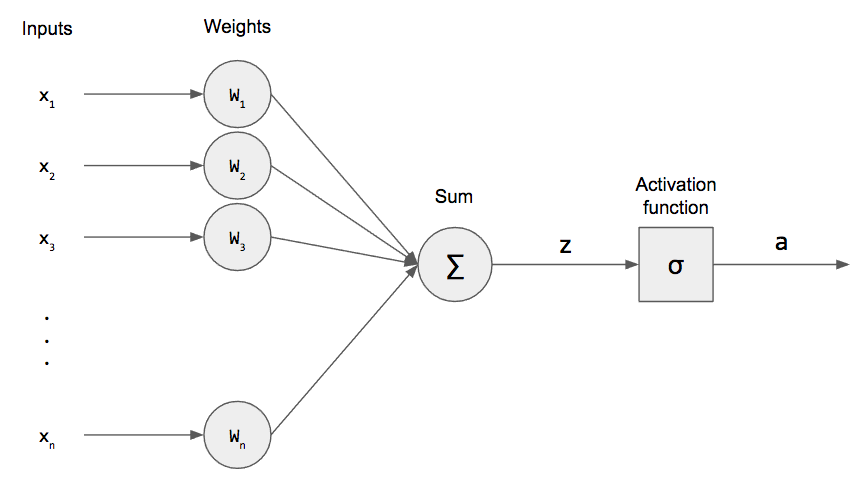
\includegraphics[width=0.8\linewidth]{images/perceptron}
\caption{Entradas, pesos, produto escalar e função de ativação.}
\end{figure}
\end{frame}

\begin{frame}
\frametitle{Funções de Ativação}

\begin{columns}[c] % The "c" option specifies centered vertical alignment while the "t" option is used for top vertical alignment

\column{.5\textwidth} % Right column and width
Dada uma entrada, define um estado para um neurônio.

\column{.45\textwidth} % Left column and width
\textbf{Tipos}
\begin{enumerate}
\item Step Function.
\item Linear.
\item Sigmoid.
\item Hyperbolic Tangent.
\item ReLU.
\end{enumerate}
\end{columns}

\end{frame}

\begin{frame}
\frametitle{Funções de Normalização}
\begin{columns}[c]
    \column{.5\textwidth}
    \begin{enumerate}
        \item Normaliza entre 0 e 1 as saídas dado um problema multi-classes processado por um neurônio.
        \item É aplicada na camada de saída (output layer).
        \item Tem como objetivo encaixar a saída obtida dentro de uma classe presente em um conjunto de classes previamente estabelecido.
    \end{enumerate}
    \column{.45\textwidth}
    \begin{figure}
        \[f(v_i) = \displaystyle\frac{e^{v_i}}{\displaystyle\sum_{j} e^{v_j}}\]
        \caption{Função softmax.}
    \end{figure}
\end{columns}
\end{frame}

\section{Convolução e Pooling}

\begin{frame}
\frametitle{Convolução}
    \begin{itemize}
        \item Operação matemática entre duas funções \textit{f} e \textit{g}, produzindo uma terceira função, que pode ser interpretada como uma função modificada de \textit{f}.
        \item Input (imagem) X Kernel.
        \item Gera Feature Maps.
    \end{itemize}
\end{frame}

\begin{frame}
\frametitle{Convolução}
    \begin{columns}[c]
        \column{.5\textwidth}
        \begin{figure}
        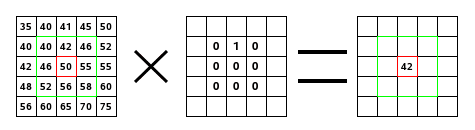
\includegraphics[width=0.9\linewidth]{images/convolution-calculate}
        \caption{Operação de Convolução.}
        \end{figure}
        \column{.45\textwidth}
        \begin{figure}
        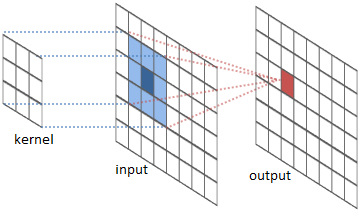
\includegraphics[width=0.9\linewidth]{images/diagram-conv}
        \caption{Relação entre o kernel e a entrada.}
        \end{figure}
    \end{columns}
\end{frame}

\begin{frame}
\frametitle{Pooling}
\begin{columns}[c]
\column{.5\textwidth}
\begin{itemize}
\item Operação de Agregação.
\item Downsampling.
\item Redução de escala através de Convolução.
\item Max, Avg, Mediana.
\end{itemize}
\column{.6\textwidth}
\begin{figure}
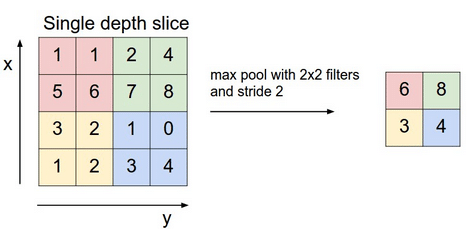
\includegraphics[width=0.8\linewidth]{images/pooling}
\caption{Pooling de Máximo.}
\end{figure}
\end{columns}
\end{frame}

\section{Deep Learning}

\begin{frame}
\frametitle{Deep Learning}
\begin{itemize}
\item Estudar um dia antes da prova == Shallow Learning (Aprendizado Raso).
\item Estudar todo dia desde o início da disciplina == Deep Learning (Aprendizado Profundo).
\item Maior quantidade de dados e processamento em GPU.
\end{itemize}
\end{frame}

\begin{frame}
\frametitle{Deep Learning}
\begin{itemize}
\item Representação em mais níveis de abstração e maior complexidade de classificação.
\item Quanto maior quantidade de dados para o treino e mais épocas, maior o aprendizado.
\item Visão Computacional, Processamento de Áudio, Big Data.
\end{itemize}
\end{frame}

\subsection{Convolutional Neural Networks}

\begin{frame}
\frametitle{Convolutional Neural Networks}
\begin{itemize}
\item Inspiradas no modelo biológico da visão.
\item Camadas de Convolução e Pooling.
\item LENET-5 (Yann LeCun, 1998).
\item Veio a ter popularidade a partir de 2006 por conta das GPUs.
\item Crescimento do uso a partir de 2010 por conta da disponibilidade de grandes massas de dados.
\end{itemize}
\end{frame}

\begin{frame}
\frametitle{Camadas de uma CNN}
\begin{figure}
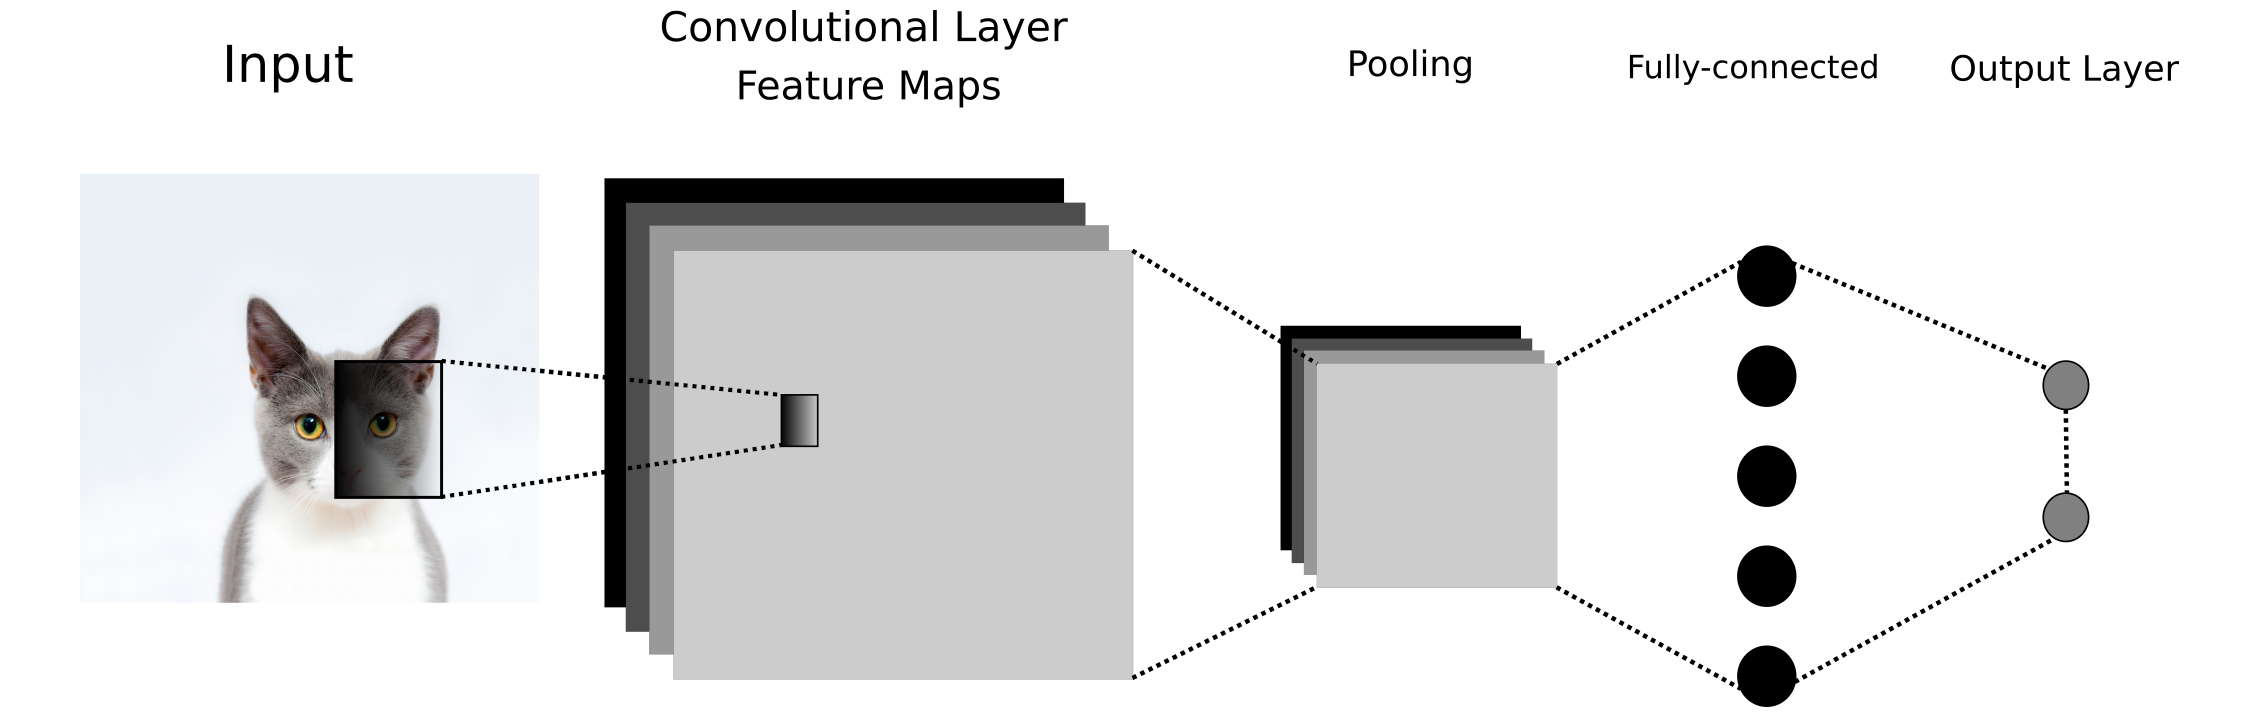
\includegraphics[width=1\linewidth]{images/cnn}
\caption{Camada de entrada, camada convolucional, camada de pooling, camada fully-connected (densa), camada de saída.}
\end{figure}
\end{frame}

\subsection{Generative Adversarial Networks}

\begin{frame}
\frametitle{Generative Adversarial Networks}
\begin{itemize}
\item Generative
\begin{itemize}
\item Aprenda um modelo generativo.
\end{itemize}
\item Adversarial
\begin{itemize}
\item A rede é treinada juntamente com uma outra rede adversária, aprendendo a partir de uma competição.
\end{itemize}
\item Networks
\begin{itemize}
\item Redes de Aprendizado Profundo.
\end{itemize}
\end{itemize}
\end{frame}

\begin{frame}
\frametitle{Generative Adversarial Networks}
\begin{itemize}
\item Ian Goodfellow et al, 2014.
\item Gerador contra Discriminador.
\item Gerador irá gerar dados a partir de um dataset inicial.
\item Discriminador irá avaliar esses dados de acordo com o dataset inicial.
\end{itemize}
\end{frame}

\begin{frame}
\frametitle{Arquitetura GANs}
\begin{figure}
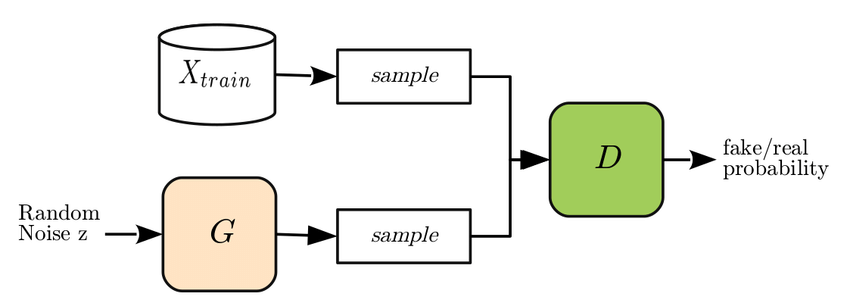
\includegraphics[width=1\linewidth]{images/gan}
\caption{Gerador procura aproximar o ruído inicial de uma imagem real, enquanto que o Discriminador avalia com base nos dados reais.}
\end{figure}
\end{frame}

\begin{frame}
\frametitle{Aplicações com GANs}
\begin{itemize}
\item Geração de imagens e dados.
\item Super resolução de imagens.
\item Recuperação de imagens.
\item Extração de objetos presentes numa imagem.
\item Texto para imagem.
\item Detecção de anomalias.
\end{itemize}
\end{frame}

\subsection{Autoencoders}

\begin{frame}
\frametitle{Autoencoders}
\begin{itemize}
\item Aprendizado não-supervisionado.
\item Tenta aprender uma função de identidade.
\item Comprime a entrada e tenta descomprimir para que a saída seja igual a ela.
\item $y^{(i)} = x^{(i)}$
\end{itemize}
\end{frame}

\begin{frame}
\frametitle{Arquitetura Autoencoders}
\begin{figure}
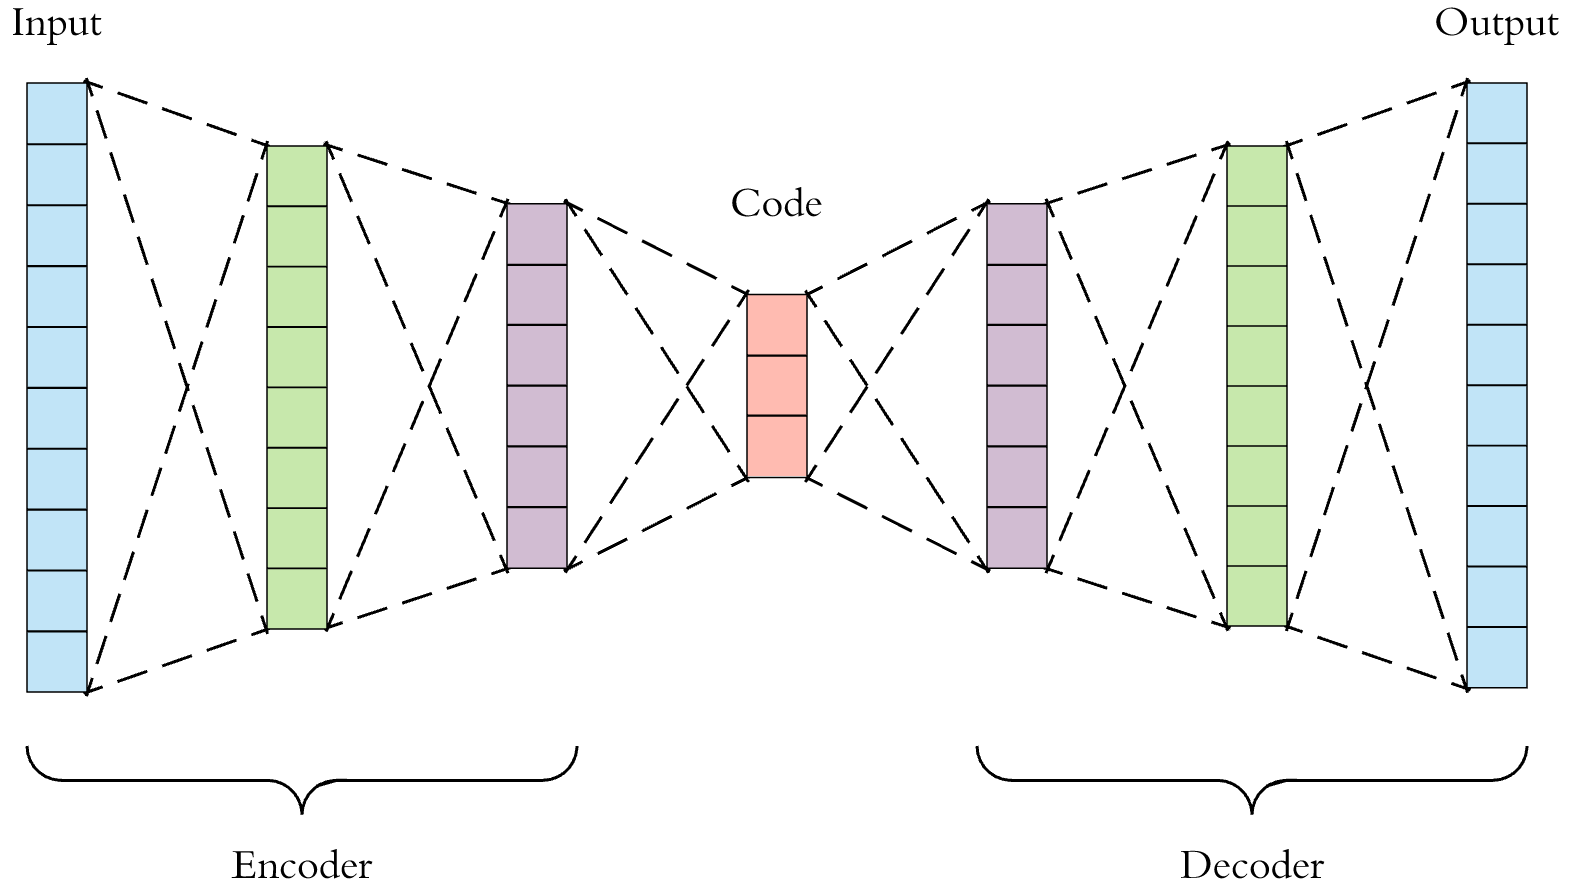
\includegraphics[width=0.9\linewidth]{images/autoencoder}
\caption{Encoder irá comprimir os dados, enquanto que o Decoder irá descomprimir.}
\end{figure}
\end{frame}

\section{Keras}

\begin{frame}
\frametitle{Biblioteca Keras}
\begin{itemize}
\item Biblioteca de alto nível para Deep Learning.
\item Feita em Python.
\item Tensorflow ou Theano como backends.
\end{itemize}
\end{frame}

\begin{frame}
\frametitle{Fluxo no Keras}
\begin{figure}
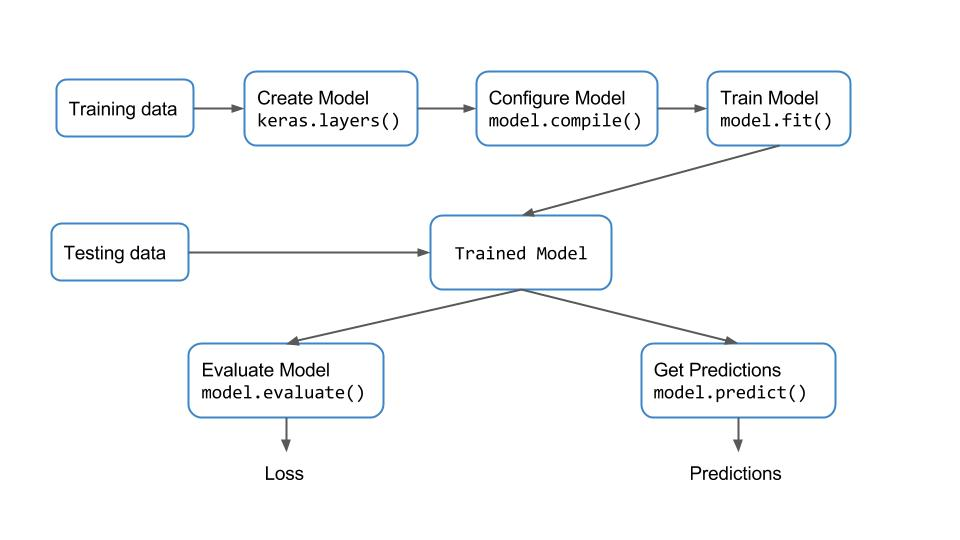
\includegraphics[width=0.9\linewidth]{images/keras-flow}
\caption{Relação entre o treino e teste no Keras.}
\end{figure}
\end{frame}

\begin{frame}
\frametitle{Camadas presentes no Keras}
\begin{itemize}
\item Dense (keras.layers.Dense).
\item Activation (keras.layers.Activation).
\item Dropout (keras.layers.Dropout).
\item Flatten (keras.layers.Flatten).
\item Convolution layer (keras.layers.Conv2D).
\item Pooling layer (keras.layers.MaxPooling2D).
\item Upsampling layer (keras.layers.UpSampling).
\end{itemize}
\end{frame}

\begin{frame}
\frametitle{Criando modelo}
\pythonexternal{code/model.py}
\end{frame}

\begin{frame}
\frametitle{Treinando modelo}
\pythonexternal{code/train.py}
\end{frame}

\begin{frame}
\frametitle{Testando modelo}
\pythonexternal{code/test.py}
\end{frame}

\begin{frame}
\frametitle{Projetos em Keras}
\begin{itemize}
\item How Are You: \href{https://github.com/cjlcarvalho/how-are-you}{cjlcarvalho/how-are-you}
\item ulcer-image-segmentation: \href{https://github.com/cjlcarvalho/ulcer-image-segmentation}{cjlcarvalho/ulcer-image-segmentation}
\item Perceptron: \href{https://github.com/cjlcarvalho/hands-on-ann/blob/master/perceptron_keras/perceptron.py}{cjlcarvalho/hands-on-ann/perceptron\_keras}
\end{itemize}
\end{frame}

%------------------------------------------------

\begin{frame}

\Large{\centerline{\textbf{Perguntas?}}}\\

\centerline{\url{https://github.com/cjlcarvalho}}

\end{frame}

%----------------------------------------------------------------------------------------

\end{document}
